\section{Implementation}

%%% SUGGESTION: For conference review, this section should read less like a narrative and more like a reproducible model specification.
%%% SUGGESTION: Recommended order:
%%% SUGGESTION: (1) topology and layer sizes,
%%% SUGGESTION: (2) orientation/layer indexing,
%%% SUGGESTION: (3) adjacency and weight masks,
%%% SUGGESTION: (4) forward pass,
%%% SUGGESTION: (5) training/update rule,
%%% SUGGESTION: (6) computational complexity,
%%% SUGGESTION: (7) implementation notes.
%%% SUGGESTION: Existing ensemble variants near the end may fit better in Benchmark Families or Future Work unless they are experimentally evaluated.

\subsection{Topological Definition}
A one directional view hexagonal neural network is a multilayer perceptron network whose layer sizes increase and then decrease symmetrically, forming a hexagon-like outline if it were to be drawn in 2D.
As expected, all neurons in any given layer are fully connected to all neurons in the subsequent layer.
However, due to the hexagonal nature of the framework, there are three distinct directions in which one could perform traditional forward and backward neural network propagation.
This renders the structure to contain a unique corresponding arrangement of connections and shared weights given the direction.

%%% SUGGESTION: Existing text: "three distinct directions"
%%% SUGGESTION: Clarify early that there are six orientations but three geometric axes if opposite directions share/reverse weights.
%%% SUGGESTION: Reviewers may otherwise see an inconsistency between "three distinct directions" and later $H_0, \ldots, H_5$.

These shared weights may influence the internal network's representation of data in their high-dimensional embedding from one propagation direction to another in strange ways.
The shared weights of, say, the first semantic layer of $H_1$ will always have at least one shared weight with $H_2$ (the relative leftmost neuron from $H_2$'s point of view) up until the halfway point of the network.
This overlap is small but non-neglible as these weights are now subject to the gradient descent paths of two distinct target local optimas.
Experimentally, we actually see equivalent or better another local optimum, outperforming the two original networks had they been started with the same random seed patterns for their respective weights across the benchmark set (detailed below).
Since each layer represents a layer of abstraction away from the input reality towards the target reality, it could be speculated that any one layer's abstraction has a cross abstractive coherence bias on another's direction and thus representation.

%%% SUGGESTION: Existing text: "strange ways"
%%% SUGGESTION: Replace with a measurable term such as "transfer", "interference", or "cross-orientation coupling".
%%% SUGGESTION: Existing text: "two distinct target local optimas"
%%% SUGGESTION: This is technically risky. Local optima claims are difficult to substantiate without loss landscape analysis.
%%% SUGGESTION: Consider describing this as "distinct optimization trajectories" unless you actually measure optima.
%%% SUGGESTION: Existing text: "Experimentally, we actually see..."
%%% SUGGESTION: Move empirical claims out of Implementation and into Results, then cite figure/table/run identifiers there.

\subsection{The Greek Stuff}

%%% SUGGESTION: Rename this subsection before submission.
%%% SUGGESTION: Options: "Formal Topology", "Layer-Size Definition", or "Notation and Geometry".

The layer sizes of a HexNet of a parameter size $n$ follow an explicit pattern:

\[L = [n, n+1, ... 2n-1, ..., n+1, n]\]

with a $2n-1$ total layers as well.
The total number of nodes in a network, however, is:

\[T = \sum_{k=0}^{2n-2} (n + \min(k, 2n-2-k))\]

%%% SUGGESTION: Consider adding the closed form $T = 3n^2 - 3n + 1$ if correct for your topology.
%%% SUGGESTION: This helps reviewers quickly reason about scaling.
%%% SUGGESTION: Also add parameter-count equations for:
%%% SUGGESTION: - one orientation path,
%%% SUGGESTION: - dense global matrix representation,
%%% SUGGESTION: - parameter-matched MLP baseline.

\subsubsection{Weight Indexing and Layer Sets}

To be explicit, if we visualize the network with the layers centered and stacked vertically (i.e. with the smallest layers at the top and bottom, widest in the middle), then we have the following directions:
\begin{itemize}
    \item \textbf{$H_0$:} Top-to-bottom layers (default hexagonal structure)
    \item \textbf{$H_1$:} Top-right to bottom-left diagonal
    \item \textbf{$H_2$:} Bottom-right to top-left diagonal
    \item \textbf{$H_3$:} Bottom-to-top layers (reverse of $H_0$)
    \item \textbf{$H_4$:} Bottom left to top-right diagonal
    \item \textbf{$H_5$:} Top left to bottom-right diagonal
\end{itemize}

%%% SUGGESTION: Verify this orientation labeling matches your code and figures exactly.
%%% SUGGESTION: Inconsistency between diagrams, code, and notation will be heavily punished by reviewers.
%%% TODO: add a table mapping orientation labels to code rotation IDs and geometric direction.

\subsubsection{Global W}

For mathematical simplicity, we employ a global weight matrix $W$, a adjacency matrix of size $T x T$ that can represent all possible connections regardless of rotation.
Given that $H_0$ is directionally opposite $H_4$, they would share exactly the same weights.
While empirical trials on MLPs show that bidirectional training on the same weights show catastrophic loss, (find reference), we could theoretically use different cells to represent that as a separate network and still maintain directional-abstraction bleeding between immediately neighboring dimensions.
If this were the case, then $W$ would not be symmetric.
An example of this is shown in Figure \ref{fig:hexnet_n3_multi_activation}.

%%% SUGGESTION: Existing text: "$H_0$ is directionally opposite $H_4$"
%%% SUGGESTION: Earlier notation says the opposite orientation of $H_i$ is $H_{(i+3) \bmod 6}$, which would make $H_3$ opposite $H_0$.
%%% SUGGESTION: This needs correction before submission.
%%% SUGGESTION: Existing text: "bidirectional training on the same weights show catastrophic loss"
%%% SUGGESTION: This needs either a citation, a specific experiment, or removal. It currently reads as an unsupported empirical claim.
%%% SUGGESTION: Existing text: "directional-abstraction bleeding"
%%% SUGGESTION: Consider replacing with "cross-orientation parameter coupling".

\begin{figure}
    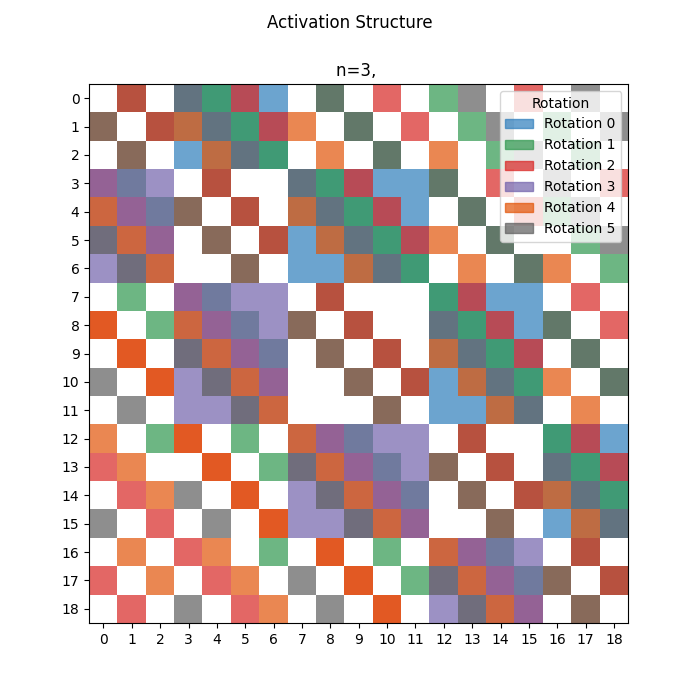
\includegraphics[width=1\linewidth]{hexnet_n3_multi_activation.png}
    \caption{Overlay of the orientation-specific adjacency patterns for a HexNN with n=3. Each color corresponds to one directed orientation.}
    \label{fig:hexnet_n3_multi_activation}
\end{figure}

\subsubsection{Directional W}
We can represent the static MLP view of any arbitrary rotation, $r \in {0, 1, 2, 3, 4, 5}$ as $W_i$ with a mask over $W$ enforcing a layered feedforward structure.

%%% SUGGESTION: Use $r \in \{0,1,2,3,4,5\}$ instead of $r \in {0, 1, 2, 3, 4, 5}$ for LaTeX correctness.
%%% SUGGESTION: Also clarify whether $W_i$ should be $W_r$, $W^{(r)}$, or $A^{(r)} \odot W$.

For the next few mathematical definitions, let the \textbf{Vertical Direction} orientation of the network, $H_1$, be the assumed direction.
Furthermore, let's assume the numbering of the network to start from the top left index, traverse left to right, and then top to bottom.
Let:
\begin{itemize}
    \item $A^{i} \in \{0, 1\}^{T \times T}$ be the binary adjacency matrix for arbitrary direction $H_i$
    \item For node index $i \in [0, T-1]$, let $\mathrm{layer}(i)$ map it to its layer number $l \in [0, N_{L}-1]$
    \item $S_{l}$ be the set of indices in layer $l$
\end{itemize}

%%% TODO: define $N_L$ before first use.
%%% TODO: define whether $A^i$ is directed or symmetric.
%%% TODO: define whether $W$ stores all possible directed edges or only canonical undirected edges.

\subsubsection{Directions as Rotations}
As previously noted, properties such as layer sizes and layer weights for $H_i$ will be the reverse for the geometric opposite network, $H_{(i+3) \bmod 6}$, and therefore, adjacency matrices, weight matrices, and other relevant matrices can all be considered symmetric (or at least will be in this paper).
But this now introduces rotation as a potentially active participant in the training steps.
Thus, for forward propagation, you can just iteratively compute:

\[x_{t+1} = R_k(f_d(W^T \times p_d(x_t)))\]

where $x_t$ is the latent vector at step $t$, $f_d$ is the hex net forward propagation through direction $d$, $R_k$ is the rotation operator at $k$, the selected rotation step, and $p_d is merely a padded mapping of x$

%%% SUGGESTION: This equation reads like a recurrent/orbit formulation, not the core feedforward implementation.
%%% SUGGESTION: If recurrence is not central to this conference paper, consider moving this to Future Work or clearly labeling it as optional rotational iteration.
%%% SUGGESTION: Existing text: "$p_d is merely a padded mapping of x$"
%%% SUGGESTION: Missing math delimiter around $p_d$ and $x$; also "merely" can be removed for technical tone.
%%% TODO: define the actual feedforward equation for a single orientation separately from iterative rotation experiments.

\subsubsection{Adjacency Matrices}

Then, the $H_1$, the only non-zero entries in $A$ are defined as:

\[A_{ij}=\begin{cases}
    1 & i \in S_{l}, j \in S_{l+1}, \text{ for some } l \in [0, N_L-2]\\
    0 & \text{otherwise}
\end{cases}\]

A symptom of this definition for $H_1$ is a block structure that gets created inside $A^1$.
Each block $(l, l+1)$ is a dense matrix of ones with size $\left|S_l\right| \times \left| S_{l+1}\right|$
Thus, $A^1$ can be visualized as:

\[
A^1 =
\begin{bmatrix}
    0 & B_0 & 0 & \dots & 0 \\
    0 & 0 & B_1 & \dots & 0 \\
    \vdots & \vdots &\vdots & \ddots & \vdots \\
    0 & 0 & \dots & 0 & B_{N_{L}-2} \\
    0 & 0 & \dots & 0 & 0
\end{bmatrix}
\]

where every $B_k \in \{0,1\}^{\left|S_k\right| \times \left|S_{k+1}\right|}$ is a matrix of all 1s.
We can see this pattern hold as $n$ grows for $H_1$ in \ref{fig:adj-matrix-n234}

%%% SUGGESTION: Add "Figure" before \ref{fig:adj-matrix-n234}.
%%% SUGGESTION: Specify whether this block matrix is shown after ordering nodes by orientation-specific layer index.
%%% SUGGESTION: Without that clarification, reviewers may wonder why the adjacency is block-upper-triangular for every rotation.

\begin{figure}
    % \centering
    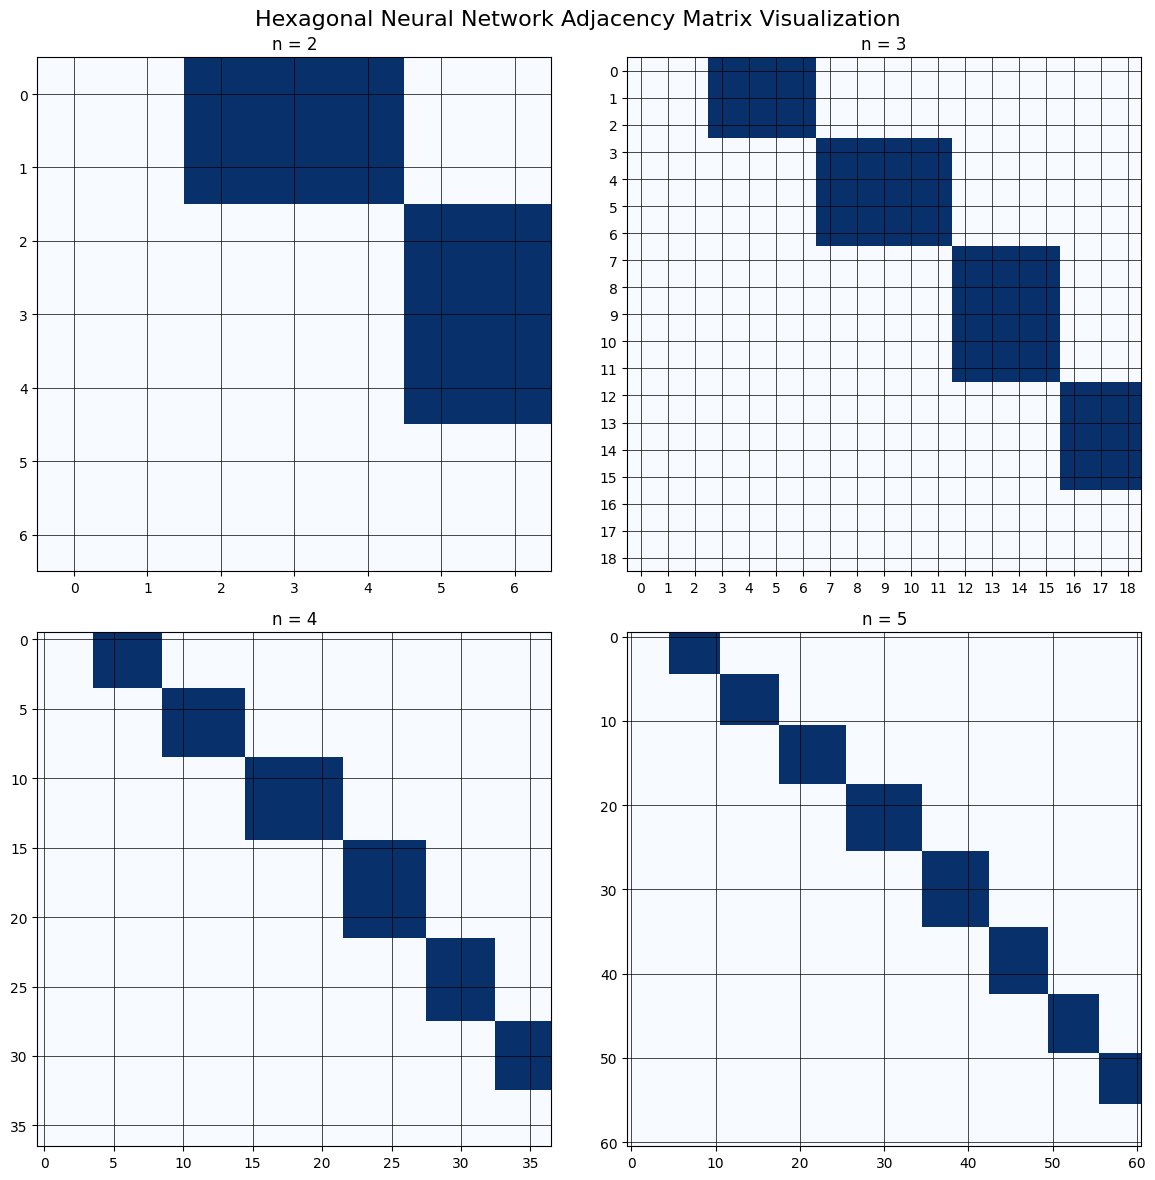
\includegraphics[width=1\linewidth]{adj-matrix-for-h1-on-n234.png}
    \caption{Adjacency Matrix showcasing the Block structure for $H_1$}
    \label{fig:adj-matrix-n234}
\end{figure}

\subsubsection{Example Training Step Flow with $n=2$}

In a network with $n=2$,
\begin{itemize}
    \item The layer sizes are $[2, 3, 2]$
    \item The total number of nodes is $T = 7$
    \item The Weight and Adjacency matrices $A, W \in \mathbb{R}^{7 \times 7}$
    \item The padded input vector $p_0(x)$ is
    \[x_t = \begin{bmatrix}
        x_0 \\
        x_1 \\
        0 \\
        0 \\
        0 \\
        0 \\
        0 \\
    \end{bmatrix}\]

    \item And the padded response vector is
    \[\text{calculated } y_t = \begin{bmatrix}
        0 \\
        0 \\
        0 \\
        0 \\
        0 \\
        y_0 \\
        y_1 \\
    \end{bmatrix}\]
    
\end{itemize}

%%% TODO: add pseudocode for one training step.
%%% TODO: explicitly state optimizer, loss, activation, batching, seed behavior, and update schedule.
%%% TODO: define how gradients on shared weights are accumulated or synchronized.
%%% SUGGESTION: A small Algorithm environment would substantially improve reviewability here.

\subsection{Computational Complexity}

%%% TODO: add asymptotic and practical complexity discussion.
%%% TODO: compare dense global matrix implementation versus block/path implementation.
%%% TODO: include memory complexity for $W \in \mathbb{R}^{T \times T}$ and active orientation blocks.
%%% SUGGESTION: This section is important because the architecture scales badly if represented as dense global matrices.

\subsection{Implementation Reproducibility}

%%% TODO: specify codebase, random seeds, software dependencies, and hardware used for reported runs.
%%% TODO: specify whether results were generated from NumPy reference implementation or another backend.
%%% TODO: specify saved run manifest fields needed to reproduce results.

\subsection{Baseline and Variant Definitions}

%%% SUGGESTION: The following baseline/variant ideas are useful, but they currently read as future experiment notes rather than implemented methods.
%%% SUGGESTION: For a conference paper, either:
%%% SUGGESTION: - move unevaluated variants to Future Work, or
%%% SUGGESTION: - convert this into a clear baseline-definition subsection and only list evaluated baselines.

If we interpret six co-dependent multi layer perceptrons as an ensemble with parameter tying, here are a few variants that we could try finding baselines within the guidance of ensemble based learning \cite{lakshminarayanan2017deep,huang2017snapshot,izmailov2018swa,gal2016dropout}.

We will establish some baseline models, and their expected outputs.
Then we will try five variants of these baselines that are based on exploits and manipulations that we can do exclusively because of hexagonal nature of the graph.
To these five, we will then be testing some orthogonal knobs.  We will establish what are the independent and dependent  and testing variables that we will be fine tuning and sweeping through to test.

First, let's establish some baselines.

\subsubsection{Baselines}

A single model, without sharing, standard training
Deep ensemble, six separate networks, no sharing, independent seeds.
Snapshot ensemble / SWA: 1 network, multi snapshot averaging
MC-Dropout: 1 net, inference-time dropout

%%% TODO: Convert this into a table with columns: baseline, parameter sharing, parameter count, trained orientations, inference rule, purpose.
%%% SUGGESTION: Parameter-count parity should be explicit for every baseline.

\subsubsection{Variants 1 - 5: Hex Ensemble Variants}
Variant 1: Hard Rotation Sharing:
One backbone tensor bank, each member 'applies a hex rotation' to filters adjacency before its forward.
Only small member-specific heads (and optional tiny offsets) are unique.
Combines group equivariance with ensembling

Variant 2: Soft sharing via low-rank delta (LoRA-style)
Shared backbone $\theta$; each member has $\Delta_i = A_iB_i$ (rank-r) on selected layers \cite{hu2022lora}.
Control r to trade diversity vs. parameters
Optimal: permember BN/Layer Norm

Variant 3: Masked weight reuse
Shared tensor bank W; each member uses a binary/ternary mask $M_i$ (learned or fixed) such that $W \circ M_i$
Encourages orthogonal subspaces with negligble memory

Variant 4: Shared backbone, member heads only
Classic multi head: 100 percent sahred feature extractor; six heads (Acts as lower bound on diversity)

Variant 5: Optimizer state-sharing vs isolatioin
Same weights but either (i) one optimizer for all members (cotraining) or (ii) per member optimizers on their delta/heads only.

%%% SUGGESTION: These variants are potentially too many for the first conference paper.
%%% SUGGESTION: A tighter paper may only need:
%%% SUGGESTION: - HexNN single-orientation baseline
%%% SUGGESTION: - parameter-matched MLP
%%% SUGGESTION: - six independent MLPs / ensemble baseline
%%% SUGGESTION: - rotation-scheduled HexNN
%%% SUGGESTION: Leave LoRA/masked/head-only variants to future work unless results already exist.
